% AER-Article.tex for AEA last revised 22 June 2011

% \documentclass[AER]{AEA} modified for the full path to my AEA.cls file
    \documentclass[AER]{./aea-latex-templates/AEA}

        \usepackage{tikz}
        \usetikzlibrary{calc,matrix}
        
        % The mathtime package uses a Times font instead of Computer Modern.
        % Uncomment the line below if you wish to use the mathtime package:
        % \usepackage[cmbold]{mathtime}
        % Note that miktex, by default, configures the mathtime package to use commercial fonts
        % which you may not have. If you would like to use mathtime but you are seeing error
        % messages about missing fonts (mtex.pfb, mtsy.pfb, or rmtmi.pfb) then please see
        % the technical support document at 
        % for instructions on fixing this problem.
        
        % harvard for bibtex, recommended by AEA
        \usepackage[abbr]{harvard}
        % booktabs for tables, recommended by https://tex.stackexchange.com/a/59035/197312
        \usepackage{booktabs}
        
        % This command determines the leading (vertical space between lines) in draft mode
        % with 1.5 corresponding to "double" spacing.
        \draftSpacing{1.5}
        
        % allowing images as figures
        % ref: https://tex.stackexchange.com/questions/19176/how-to-insert-an-image-into-latex-document
        \usepackage{graphicx}
        \graphicspath{{./figures-and-tables}}
        
        \usepackage{hyperref}
        
        \begin{document}
        
        \title{Attitudinal Trends in Alternative Postsecondary Learning
            \thanks{
                Go to \url{https://papers.ssrn.com/sol3/papers.cfm?abstract_id=3387110} to visit
                the article page for additional materials including the online appendix,
                survey data, and data analysis source code.
            }
        }
        \shortTitle{Trends in Alternative Learning}
        \author{John Vandivier
            \thanks{
                    Vandivier: George Mason University,
                    4400 University Dr, Fairfax, VA 22030,
                    jvandivi@masonlive.gmu.edu.
                    The author acknowledges valuable input from Bryan Caplan at George Mason University.
                }
            }
        \date{\today}
        \pubMonth{Month}
        \pubYear{Year}
        \pubVolume{Vol}
        \pubIssue{Issue}
        \JEL{D12, I21, I22, I24, I25, I26}
        \Keywords{Education economics, alternative education, debt crisis, signaling}

        \begin{abstract}
        This paper explores a novel data set (n = 1190) to understand trends in public
        disposition on alternative postsecondary learning, with a focus on employers.
        Results indicate that public favorability is positive and will remain flat over the next year.
        Employer attitudes are not meaningfully different from the general public.
        \end{abstract}

        \maketitle
        
        \section{Introduction}

        Student loan debt in the United States is the highest ever\cite{friedman2018student},
        even while accredited postsecondary education is becoming a dynamically worse investment
        for at least two reasons.

        The first reason is the plain fact that college is growing in price while adjusted return remains stagnant.
        From 1989 to 2012, K-12 student expenditure increased significantly
        \footnote{
            From 1989 to 2012, the average cost of a year of undergraduate education in the US rose 79 percent
            from \$11,862 to \$21,222 in constant 2016 dollars.
            This price includes tuition and fees plus room and board for full-time students in degree-granting postsecondary institutions.
            Data from \cite{nces2017averageundergraduatetuition}.
        },
        the cost of a year of undergraduate education grew nearly three times more quickly than that
        \footnote{
            From 1989 to 2012, per pupil public expenditure for K-12 students increased 27 percent
            from \$8,654 to \$11,011 in constant 2014 dollars. Data from \cite{nces2015expendituresperpupil}.
        },
        and the adjusted average starting salary of a college graduate decreased by about 9 percent
        \footnote{
            From 1989 to 2012, a decrease of \$4,385 from \$49,487 to \$45,102 in constant 2016 dollars is observed. (4385/49487) = 0.089.
            From 1960 to 2012, an increase from \$47,442 to \$50,219 is observed. Data from \cite{koncz2016}.
        }.

        The second reason traditional postsecondary education has become a
        weaker investment during recent years is the growth of alternatives.
        This paper fills an empirical gap in scholarly research by supplying
        systematic and general data about public and employer favorability of
        alternative credentials.
        This paper tests the hypothesis that employer favorability is positive toward alternative credentials.
        % Alternative education faces adoption problems among learners, employers,
        % and third parties such as parents and teachers which influence the former two groups.
        % Learner willingness to consume alternative education is endogenous with employer favorability and entry-level job suitability.
        % If employers are favorable, dispersion of favorability information would at once explain the growth of alternative education and also ostensibly stimulate further adoption.
        
        Alternative postsecondary learning activities are diverse and do not
        exclude attainment of an accredited degree, but may involve strategic
        delay or acceleration of accredited education when compared to traditional approaches.
        Delayed formal education improves the return to education for
        individuals who are able to leverage employer funding. Accelerated completion improves the return to education in general.
        Online education is an alternative approach which reduces the cost of college for most students
        \footnote{
            Mattern and Wyatt\cite{mattern2009student} note that college students live an average distance of
            268 miles from home and a median of 94 miles. This indicates that most students could reduce
            the cost of college by studying remotely from home.
        }.
        
        \section{Data}
        
        1190 responses, including partial responses, were obtained for four
        comparable survey administrations from February 2018 to May 2019.
        Analysis includes 114 right-hand variables and two left-hand variables.
        Appendix A details the wording of questions and possible responses.
        Appendix B identifies factors included in each administration.

        Responses were collected mainly through SurveyMonkey and Amazon Mechanical
        Turk paid response, with a non-trivial number also coming from social media
        and word of mouth. Each origination channel was grouped using a construct
        called a collector. Collector effects were insignificant. This is
        interesting for two reasons. First, the source
        populations are known to be systematically different. Amazon Mechanical Turk
        respondents, for example, were guaranteed to be U.S. High School graduates. A second
        reason the insignificance of collector effects is important is that
        response prices were significantly different. Amazon Mechanical Turk
        responses were more than 20 percent cheaper than SurveyMonkey Paid Audience
        responses on average.
        
        Factor-level sample size ranges from 240 to 1190. Appendix C lists
        technical variable names in alphabetical order along with summary
        statistics. Appendix D lists variable names in alphabetical order, and
        summarizes factor strength across models.
        Several constructs, such as income, age, and gender, were redundantly
        operationalized using different measures. For example, age was measured
        continuously and also by age group. Appendix D makes this
        factor-to-variable mapping clear.
        
        The variable of interest is entry-level suitability.
        This variable corresponds to question 2 in Appendix A.
        It is structured as a favorability question on a scale from 1 to 10. Higher numbers indicates stronger agreement.
        The wording of the statement to be favored is, "For many professions, alternative credentials can qualify a person for an entry-level position."
        
        A secondary variable of interest explored is called the index of interest.
        This is a 3-factor index of similar but different favorability questions.
        This variable was checked to ensure findings are robust to the specic wording of the primary variable of interest.
        This variable also includes a question on online learning. As a result, findings are more broadly generalizable
        to alternative education, rather than alternative credentials in particular.
        
        No survey administration allowed for measurement of all variables simultaneously,
        but within each calender year ordinary least squares modelling identified four key models.
        Analysis of survey results from 2018 indicated that certain factors were unimportant.
        As a result, some questions were replaced in 2019.

        The 2019 analysis covers the whole data set, not only samples from 2019.
        Questions in the October 2018 administration are a superset of those in February 2018.
        Similarly, May 2019 variables are a superset of February 2019.
        It turns out that the most significant factors identified in the
        2019 analysis were also measured in the 2018 administrations, but this may be due to oversampling.
        
        The first key model is a long model using all available right hand variables.
        Factors are eliminated one at a time until a subsequent key model is obtained.
        The second key model is the weak model. This model includes factors with a p-value of less than .5.
        The third model is an adjusted r-squared maximizing model, and the fourth
        model is a strong model involving factors with a p-value less than .1.

        \section{Empirical analysis and results}

        The average response for the variable of interest was 6.61.
        The median response was 7 and the 25th percentile was 5.
        This indicates uncorrected broad positive sentiment.
        Unemployed status and identification with the ethnicity of
        other are the two largest significant effects, and they are both positive
        \footnote{
            This ignores a complex discussion on gender. 
            \ref{tab:models} indicates the effect of male identification is
            large in the preferred model, but this is attributable to the
            concurrent presence of additional, insignificant gender variables.
            Male identification is taken to have a true effect close to -0.42,
            the value identified in the strong model with higher significance.
        }.
        Employer effects are not significant in any model, although in the preferred
        model employer effects obtain a coefficient of about -.47 and a p-value of .215.

        Two negative coefficients obtain a p-value of less than 0.1, but neither effect is
        large enough over the relevant range to reduce favorability to a disfavorable
        state of less than 5. Male gender identification reduces the point estimate of the
        dependent variable by about 0.42, and the quadratic negative effect of expected
        conventionality is attenuated by a positive linear effect.

        Expected conventionality is one of three components of the secondary variable of interest, the index of interest.
        It is a favorability question on a scale of 1 to 10 about the statement,
        "It will soon become fairly conventional for high school graduates to obtain alternative credentials instead of going to college."
        The average response for this question is 6.1, which is lower than entry-level
        suitability and favorability of online education, the other two components of the index.

        The average response for favorability of online education was the highest among the three components at 6.81.
        The average response for the index was 19.55.
        All three components of the index of interest are strongly intercorrelated,
        indicating results for the entry-level suitability of alternative credentials
        in particular are importantly generalizable to alternative education in general.
        Moreover, the shape of the relation between any two of these components is
        linearly positive with decreasing marginal effects.
        Additional selected factor results are presented in \ref{tab:voi_by_is2018response}.
        Appendix D describes factor strength across all models.
        
        % commented means insignificant across all.
        \begin{table}
            \caption{Medium and Strong Models, Selected Variables}
            \begin{tabular}{lllll}
            Factor & 2018 Medium & 2018 Strong & 2019 Medium & 2019 Strong \\
            \toprule
            %Profile Female & 1.091** & 0.955** \\ % issurveymonkeyfemale
            %Profile Male &  &  & 2.162* &  \\ % issurveymonkeymale
            Male &  &  & -2.458* & -0.422** \\
            % isstem & TODO & TODO & TODO & TODO \\
            Not STEM & -1.269* \\ % isnotstem
            % isindustry1 & 1.797 \\
            % isindustry2 & 1.424* \\
            % isindustry4 & 0.960 \\
            % isindustry5 & 1.395* \\
            % isindustry6 & TODO & TODO & TODO & TODO \\
            % isindustry7 &  &  & -2.514** \\
            % isindustry10 & TODO & TODO & TODO & TODO \\
            % isindustry11 & 1.203 \\
            % isindustry12 & -1.668 \\
            % Middle Atlantic
            % \\Region & 0.834 & 0.895 & -1.214** \\ % isregion2
            % isregion3 & TODO & TODO & TODO & TODO \\
            % isregion4 & TODO & TODO & TODO & TODO \\
            % isregion6 & TODO & TODO & TODO & TODO \\
            % West South
            % \\Central Region & -1.533** & -1.531** \\ % isregion7
            Pro AI & 0.700* & 0.776** \\ % nvoifai1
            Quadratic
            \\Pro AI & -0.065* & -0.069** \\ % nvoifai2
            % Cubic Pro AI &  &  & 0.001 & 0.000* \\ % nvoifai3
            Quadratic
            \\Pro American & 0.011* & 0.011* \\ % nvoifamerican2
            Quadratic Expect
            \\Convention &  &  & 0.113** & 0.081** \\ % nvoifconventionalsoon2
            Cubic Expect
            \\Convention & 0.003** & 0.003** & -0.007* & -0.005*** \\ % nvoifconventionalsoon3
            % nvoifcrypto2 & TODO & TODO & TODO & TODO \\
            % nvoifonline1 & TODO & TODO & TODO & TODO \\
            Quadratic Pro
            \\Online Learning & 0.067 & 0.016* & 0.240 & 0.013*** \\ % nvoifonline2
            % nvoifonline3 & TODO & TODO & TODO & TODO \\
            Pro Regulation & 1.161 & 0.110* & 0.268*** & 0.110*** \\ % nvoifregulation1
            % nvoifregulation2 & TODO & TODO & TODO & TODO \\
            % nvoifregulation3 & TODO & TODO & TODO & TODO \\
            Religiosity & 0.120* & 0.105* \\ % nvoifreligion1
            % csmage1 & TODO & TODO & TODO & TODO \\
            % csmage2 & TODO & TODO & TODO & TODO \\
            % csmage3 & TODO & TODO & TODO & TODO \\
            Income & 0.770** & 0.192* \\ % csmincome1
            Quadratic Income & -0.056* &  & 0.046 &  \\ % csmincome2
            % csmincome3 & TODO & TODO & TODO & TODO \\
            % cprovider1 & TODO & TODO & TODO & TODO \\
            % cprovider2 & TODO & TODO & TODO & TODO \\
            % Cubic Time & -0.000 &  & 0.000* &  \\ % ctime3
            % ismanager & TODO & TODO & TODO & TODO \\
            Unemployed &  &  & 1.118* &  \\ % isunemployed
            % isethnicity4 & TODO & TODO & TODO & TODO \\
            Other Ethnicity &  &  & 1.682* & \\ % isethnicity6
            % ishighered & TODO & TODO & TODO & TODO \\
            % ceduc1 & TODO & TODO & TODO & TODO \\
            % ceduc2 & TODO & TODO & TODO & TODO \\
            X$_0$ & 1105.125 & .106 & -12345.347* & 3.289*** \\
            \bottomrule
            R-Squared & .597 & .504 & .526 & .319 %
        
            \end{tabular}
            \begin{tablenotes}
                * p $<$ .05
                ** p $<$ .01
                *** p $<$ .001
                Additional gender variables are excluded for simplicity.
                Industrial and regional effects are also excluded for brevity.
                Cubic effects are excluded where the significant coefficient would display as 0.000.
                Selected variables include all other variables which are significant at one of the noted levels in at least one model presented in this table.
                See the online appendix for coefficient data for further information.
            \end{tablenotes}
            \label{tab:models}
            \end{table}
        
        Overall, the 2019 medium model is preferred. This model obtains high explanatory power while maintaining relatively low complexity.
        This model explains the majority of the sample variation, with an r-squared of about .526 and an adjusted r-squared of about .44.
        Investigation of the 2018 results initially indicated weak effects for religiosity and STEM identification,
        but reanalysis with added 2019 data suggests that inclusion of these variables may add importantly to adjusted explanatory power.
        
        Innovation proxies include favorability to artificial
        intelligence, cryptocurrency, and online education. These variables are
        cross-correlated with one another with a p-value of less than .001.
        An apparent paradox is identified regarding innovation proxies.
        Favorability to government regulation is positively associated with
        innovation proxies, while religiosity is associated with reduced
        innovation favorability.
        
        Suppose a religious individual is a conservative.
        This amounts to identification status quo bias
        by conservatives, a theme common in the literature\cite{eidelman2012bias}.
        In the case of education, however, this is a bit paradoxical.
        The market is considered an effective tool of innovation\cite{baumol2002free},
        so individuals seeking to maintain the status quo ought to disfavor it rather than favor it.
        Second, traditional education is regulated education,
        so individuals committed to high levels of regulation ought to disfavor
        alternative credentials.

        A Kahneman-like explanation may reconcile this paradox.
        Survey respondents may be thinking fast\cite{kahneman2011thinking}.
        The preference of some conservatives for the status quo in education becomes explained by
        decisionmaking which is driven preferentially by
        risk aversion, loss aversion, lack of openness, and related factors.
        It may be the case that many of these same individuals would favor alternative
        credentials when a logical mode of thought is activated over fast thinking or intuition.
        
        Age group had a more robust effect compared to exact age, which may
        indicate something like a cohort effect.
        Minors are the only age group which is unfavorable toward alternative credentials on average.
        Minors have the largest share of minimum-favorability responses.
        Minors are also the least sampled group in this data set.
        
        Educational attainment obtained an important effect which was more
        significant than either age or income effects. In addition to level of
        education, a dummy variable for whether education was at or greater than
        obtaining a college degree was found to be independently significant.
        
        Three industrial effects exist in the preferred model and they are all negative.
        At -2.51, the legal industry is associated with one of the largest negative effects in any model.
        The coefficient for law is significant with a p-value of 0.006.
        The transportation industry effect is also significant with a p-value of 0.086 and a coefficient of -1.67.
        Responses of other industry are negative but insignificant, with a p-value of .294 and a coefficient of -.41.
        Three regions have effects in the preferred model, but only one is significant.
        The mid-atlantic region, including Washington DC and New York City, is associated with a coefficient of -1.21 and a p-value of 0.01.
        Regional effect robustness to the introduction of an ethnicity question in the 2019 administation supports the thesis that policy is relevant to the growth of alternative education.
        The legal and transportation industries share a common theme of licensing.
        
        Time has an unimportant effect in the preferred model.
        The standard deviation of the variable of interest is about 2.57.
        Disaggregation by year indicates a mean response of about 6.66 in 2019 and an insignificantly
        different mean of 6.35 in 2018.
        % previously called table 3 from analysis-2-basic-exploration.do; `tab is2018sample, sum (voi)`
        Modelling of suitability on time was also insignificant using logarithmic and logistic analysis,
        but a two-factor exponential expansion was discovered which forms a useful dynamic model:
        
        \begin{equation} f(x) = b_1b_2^t \end{equation}
        
        This nonlinear model obtained an adjusted r-squared of .8689 and $b_2$ had a p-value
        less than .001. The estimate of $b2$ was less than 1, indicating exponential
        decay, but the rate of decay is trivial so that forecasting is essentially flat.
        % see special reg 26
        On Monday, February 26, 2018, when $t=0$ the predicted dependent variable is equal to $b1$, which is estimated at about 6.65.
        $t$ increments by the day, and the maximum value within the sample is 437. At that time, the point estimate
        for the dependent variable is about 6.59. Forecasting a year into the future, the estimate is about 6.55.
        
        % reg voi ctime1 ctime2 managertime1 managertime2, noconstant
        A different dynamic perspective involves employer-lead favorability cycles.
        A multiple regression of four variables on the variable of interest results in an adjusted r-squared of about .8692.
        These four variables include time interacted with employer status, linear time, and the squares of each of those two.
        In this model, time has a linear negative and positive marginal coefficient, although neither are significant.
        Interacted employer-time, however, is significant, as is its quadratic variant. Linear employer-time is positive
        and the marginal effect is negative. The linear effect is about 0.002, with a p-value of about 0.03.
        The quadratic p-value is also about 0.03, but the coefficient is unimportant.
        This cycle model is conceptually depicted in Figure \ref{fig:employer_driven_favorability}.
        Population favorability exists at II and employer attitudes are represented at III.
        
        \begin{figure}[h!]
            \centering
            \caption{Employer Driven Favorability}
        
            \begin{tikzpicture}[element/.style={minimum width=1.75cm, minimum height=0.85cm}]
        
            \node (n1) [above=0.25cm] {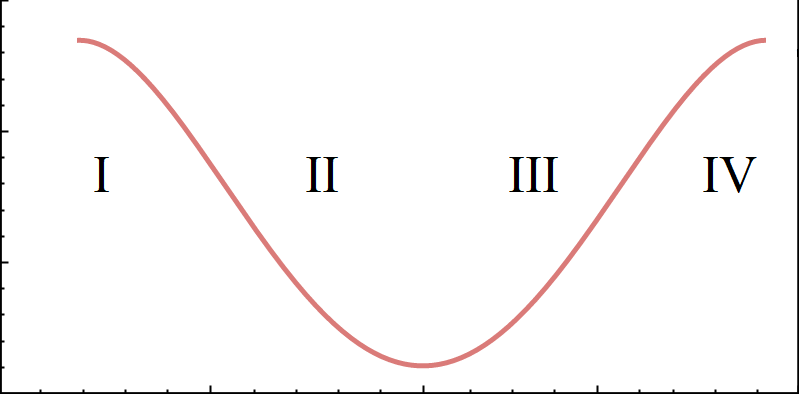
\includegraphics[width=0.7\textwidth]{./figures-and-tables/figure-4.png}};
            \node (n2) [above=0.25cm] at ($(n1)!0.5!(n1) - (6.2, 0)$) {\textbf{Suitability}};
            \node (n3) [above=0.25cm] at ($(n1)!0.5!(n1) - (0, 3.5)$) {\textbf{Time}};
        
            \end{tikzpicture}
        
            \label{fig:employer_driven_favorability}
            \end{figure}

        \section{Conclusions}
        
        Results have applications for learning providers, employers, policy, and students.
        Age effects suggest learning providers should consider marketing to parents,
        rather than directly to high school students.
        Employers tend to adopt practices from large corporations in their industry.
        Large corporations are able to leverage economies of scale, spread risk across a number of hires,
        and internally train alternatively educated individuals.
        Alternatively educated individuals are diverse\cite{florentine_2018}, and diversity is a common corporate goal.
        These incentives allow an adoption strategy which is for alternative learning providers to target large,
        industry-leading corporations.
        This movement is already taking place. Industry leaders are already disavowing the need for formal education\cite{glassdoor_2018}.

        Policymakers should level the playing field for alternative education by limiting federal grant and loan programs,
        or empowering alternative education with those dollars.
        Licensing requirements should be improved to support evidence-based competency in lieu of accredited education.
        Internship regulation should be relaxed to facilitate learning while working.
        Finally, tax write-offs and tax-privileged investment vehicles targeted at accredited education should be liberalized
        to support alternative education.

        Students should consider learning online, choosing non-elite providers,
        prior learning assessments, and credit by examination.
        For roles where a degree is inessential to junior placement, students should prefer a strategy of
        deferred college and leverage employer assistance once a role is obtained.
        
        % ref: https://www.youtube.com/watch?v=KS9GvK7cvmo
        % https://tex.stackexchange.com/a/51501/197312
        \bibliographystyle{./aea-latex-templates/aea}
        \bibliography{BibFile}
        
        \end{document}
        